\section{Regular Languages}
\subsection{Introduction}
How do we specify i.e. describe languages?
\textbf{Finite languages} Since a language is a set of words,
any finite set can be exhaustively enumerated.
\textbf{Infinite languages} An exhaustive enumeration is not possible
(in a finite time). Consequently, more general concepts are required.\\

\textbf{Regular languages} are the simplest class of languages.
Each one of these formalisms define this class of languages:
\begin{itemize}
  \item \textbf{Finite state automata}
  \item \textbf{Regular grammars}
  \item \textbf{Regular expressions}
\end{itemize}
They all have the same expression power, i.e. they all describe the same things.

\subsection{Finite State Automata}
A \textbf{finite state automaton (FSA)} consists of the following three components:
\begin{itemize}
  \item A \textbf{finite set of states} (drawn as circles).
  \item A \textbf{transition function} describing the actions which allow
        the transition from one state to another (drawn as arrows).
  \item The \textbf{initial state} i.e. the state in which the automaton is in initially 
        (indicated by an arrow coming form nowhere pointing at it). 
\end{itemize}
First, we will consider \textbf{deterministic} finite state automata (DFA) and then \textbf{non-deterministic}
finite state automata (NFA). Both DFA and NFA are FSA.\\

\textit{Example:} A switch changing alternately between two states ``ON'' and ``OFF''
can be modelled as follows:
\begin{figure}[H]
  \centering
  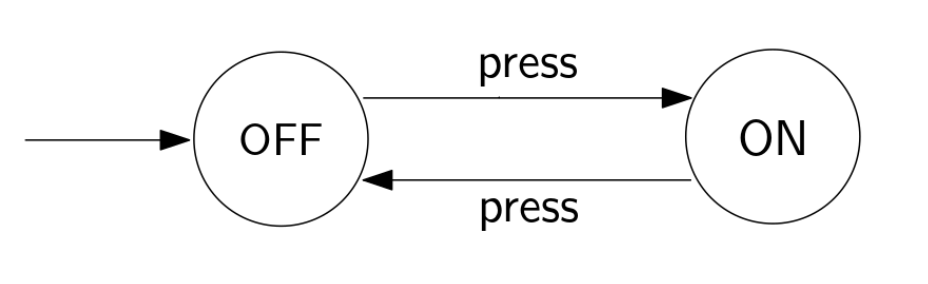
\includegraphics[width=\columnwidth]{reg-lang-1}
\end{figure}
\textit{Example:} Another example is that of a circular selector
for radio channels LW, MW and SW. This selector can be turned in any directions from LW to SW 
passing by MW, but not directly from LW to SW. Such a selector can be modeled as follows:
\begin{figure}[H]
  \centering
  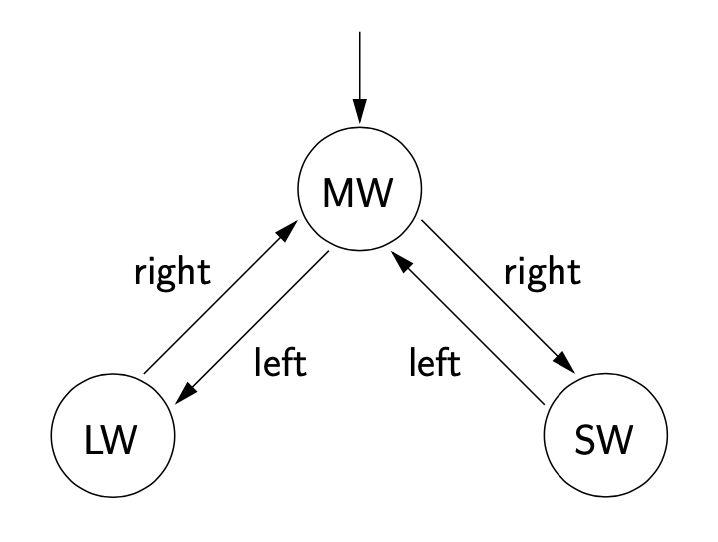
\includegraphics[width=\columnwidth]{reg-lang-2}
\end{figure}

\subsubsection{Deterministic Finite State Automata}
Deterministic finite state automata can be formally defined as being a 4-tuple $(Q, \Sigma, \delta, q_0)$, where:
\begin{itemize}
  \item $Q$ is a finite set of states
  \item $\Sigma$ is a finite set of symbols, i.e. an alphabet
  \item $\delta : Q \times \Sigma \rightarrow Q$ is a transition function
  \item $q_0 \in Q$ is the initial state
\end{itemize}

The transition function $\delta : Q \times \Sigma \rightarrow Q$ 
expresses which symbol moves the automaton from one state to the next one.
Such functions represent the transition with their label. 
Automata with an infinite number of states do not share the 
same properties with automata with finite states.\\

The extension of $\delta$ is the function $\delta^{*} : Q \times \Sigma^{*} \rightarrow Q$ 
which provides the next state for a sequence of symbols and can be defined as follows:
For a state $q \in Q$, a word $w \in \Sigma^{*}$ and a symbol $s \in \Sigma$,
the function $\delta^{*} : Q \times \Sigma^{*} \rightarrow Q$ is recursively defined as follows:
\begin{enumerate}
  \item $\delta^{*}(q, \epsilon) = q$
  \item $\delta^{*}(q, ws) = \delta(\delta^{*}(q,w),s)$
\end{enumerate}

\textit{Example:} Using the previous example with the radio, the transition function of the automaton is as follows:
\begin{align*}
  \delta(\text{MW, right}) & = \text{SW}\\
  \delta(\text{SW, left}) & = \text{MW}\\
  \delta(\text{MW, left}) & = \text{LW}\\
  \delta(\text{LW, right}) & = \text{MW}
\end{align*}
Further, the following three uses of $\delta^{*}$ are correct:
\begin{align*}
  \delta(\text{MW, left $\cdot$ right}) & = \text{MW}\\
  \delta(\text{LW, right $\cdot$ right $\cdot$ left}) & = \text{MW}\\
  \delta(\text{MW, right}) & = \text{SW}
\end{align*}

% \subsubsection{DFA Language Recognizers}
A \textbf{language recognizer} is a FSA that answers whether
a given word belongs to the language described by an automaton.
An input word is \textbf{recognized} or \textbf{accepted} by a given recognizer 
if and only if a final state is reached.
The set of all recognized words by a given recognizer forms the language modeled by the automaton 
and is called the \textbf{recognized language} by the automaton.\\

Formally defined, a DFA language recognizer is a DFA equipped with a set of final states.
Final states are drawn as double circles.
It is a 5-tuple $(Q, \Sigma, \delta, q_0, F)$ where
\begin{itemize}
  \item $Q$ is a finite set of states
  \item $\Sigma$ is a finite set of symbols, i.e. an alphabet
  \item $\delta : Q \times \Sigma \rightarrow Q$ is a transition function
  \item $q_0 \in Q$ is the initial state
  \item $F \subseteq Q$ is a set of final states
\end{itemize}
The difference between a DFA and a DFA recognizer lies only in the 
additional final states, which are included in $Q$.\\

Informally, a word is recognized by a DFA if and only if there 
exists one path from the initial state to one of the final states.
Formally, however the following definition is used:
A word $w \in \Sigma^{*}$ is recognized by a DFA $M = (Q, \Sigma, \delta, q_0, F)$
iff $\delta^{*}(q_0, w) \in F$.\\

The language recognized (or accepted) by a DFA $M$ is denoted $L(M)$. This is the set of all the words recognized by $M$.\\

Finally, we can define regular languages as follows:
Every language recognized by a finite state recognizer automaton is called a \textbf{regular language}.\\

\textit{Example:} The language 
\begin{align*}
  L_2 = \{ acbb, accbb, acccbb, accccbb, \dots \}
\end{align*}
is recognized by the following automaton:
\begin{figure}[H]
  \centering
  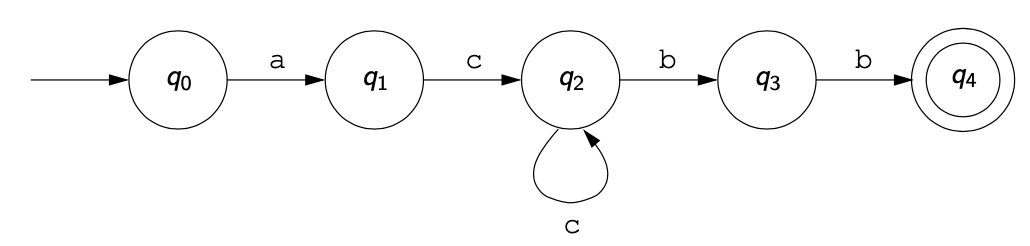
\includegraphics[width=\columnwidth]{reg-lang-3}
\end{figure}
\textit{Example:} Let $A$ be the DFA recognizer formally defined as
\begin{align*}
  A & = (Q, \Sigma, \delta, q_0, F)\\
  Q & = {q_0, q_f}\\
  \Sigma & = \{ 0,1 \}\\
  F & = {q_f}\\
  \delta(q_0, 0) & = q_0\\
  \delta(q_0, 1) & = q_f\\
  \delta(q_f, 0) & = q_0\\
  \delta(q_f, 1) & = q_f
\end{align*}
\begin{figure}[H]
  \centering
  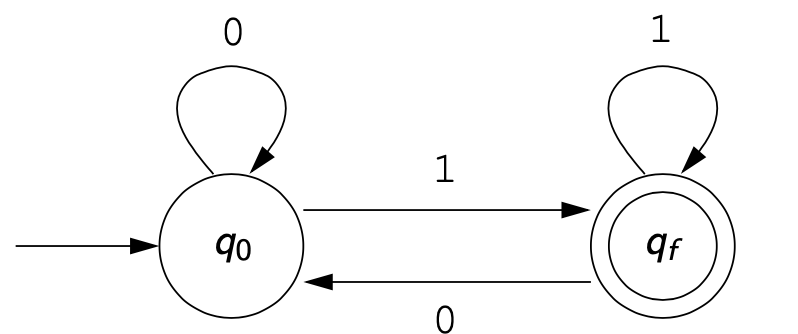
\includegraphics[width=\columnwidth]{reg-lang-4}
\end{figure}
If we consider that the words over the alphabet $\Sigma = \{0,1\}$ denote
the binary numbers, the recognized language by $A$ is 
\begin{align*}
  L(A) = \{ x \mid x \in \{0,1\}^{+} \text{ and $x$ is odd}\}
\end{align*}
\textit{Example:} Let $B$ be the DFA recognizer graphically represented by:
\begin{figure}[H]
  \centering
  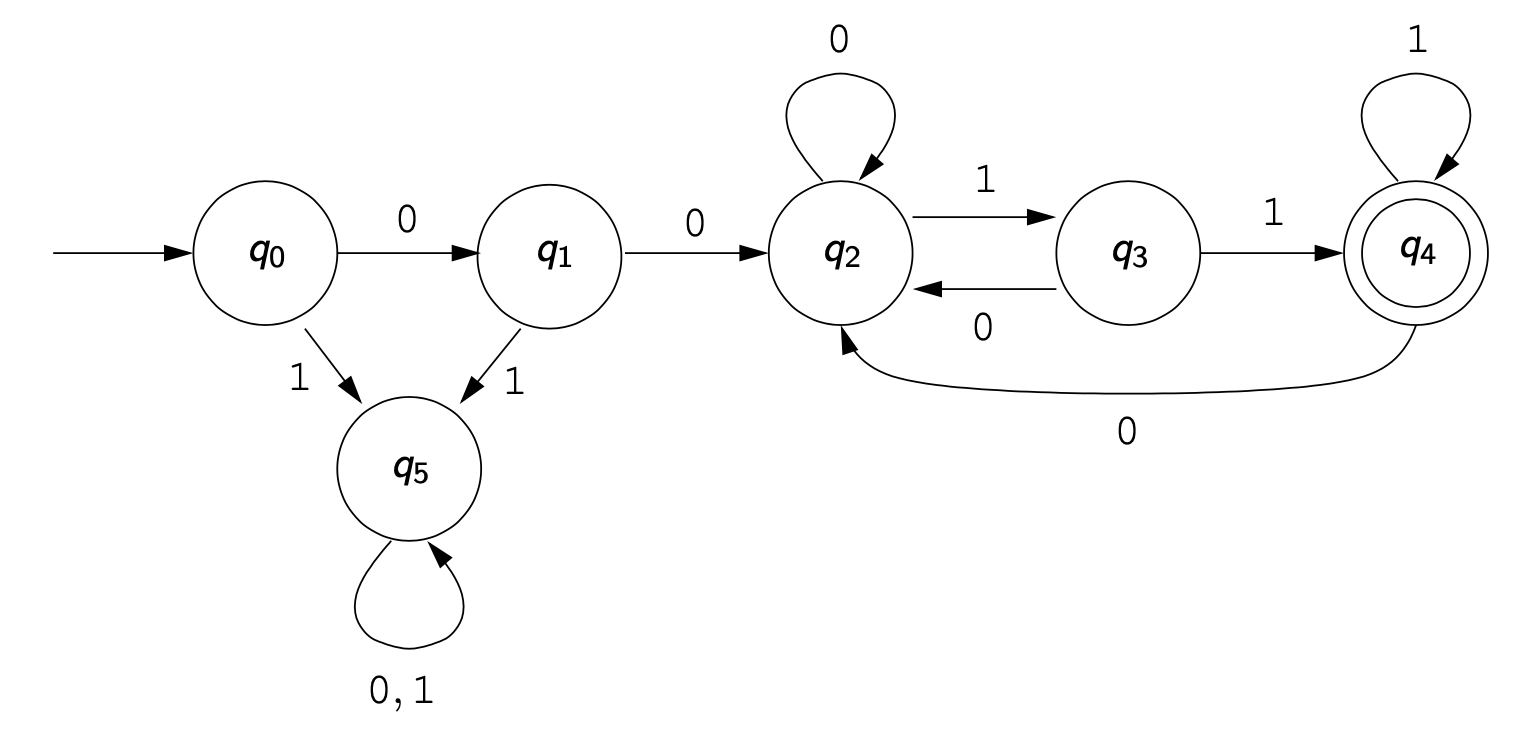
\includegraphics[width=\columnwidth]{reg-lang-5}
\end{figure}
The language recognized by $B$ is then
\begin{align*}
  L(B) = \{ 0^{n}x1^{m} \mid n \geq 2, m \geq 2, x \in \{0,1\}^{*}\}
\end{align*}
A function is called \textbf{totally defined} if it is 
defined for all possible inputs. In finite state automata, 
$\delta$ is called totally defined if it is defined for all states
and symbols.
\subsubsection{Non-deterministic Finite State Automata}
Up until now, we have seen DFA with the property
that form one state, another state can be reached in an unique manner
by $\delta$. Non-deterministic finite state automata allow multiple 
transitions from a given state and a given symbol. Finite state automata
in general can be defined as the union of DFA and NFA.\\

NFA and DFA have the same expression power. Everything that can be represented as a DFA
can also be represented as a NFA and vice versa.
The usage of non-determinism makes the automata smaller
and easier to understand.\\

Graphically, a non-deterministic choice is represented by several arrows leaving a state, 
with each arrow labeled with the same symbol.
\begin{figure}[H]
  \centering
  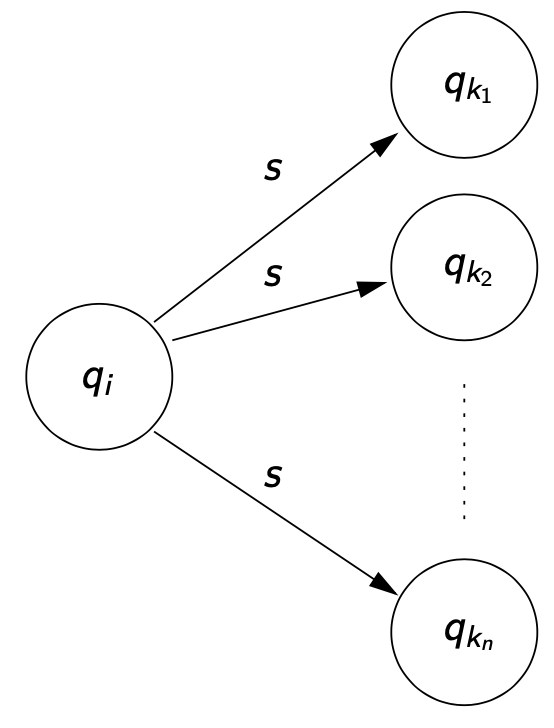
\includegraphics[width=0.5\columnwidth]{reg-lang-6}
\end{figure}
The co-domain of the transition function is the power set of the set of states $Q$:
\begin{align*}
  \delta : Q \times \Sigma \rightarrow \mathcal{P}(Q)
\end{align*}
where $\mathcal{P}(Q)$ is the power set of $Q$.\\
Formally defined, a non-deterministic automaton is a 5-tuple $(Q, \Sigma, \delta, q_0, F)$ where
\begin{itemize}
  \item $Q$ is a finite set of states
  \item $\Sigma$ is a finite set of symbols, i.e. an alphabet
  \item $\delta : Q \times \Sigma \rightarrow \mathcal{P}(Q)$ is a transition function
  \item $q_0 \in Q$ is the initial state
  \item $F \subseteq Q$ is a set of final states
\end{itemize} 
Similarly to DFA, the extension function $\delta^{*}$ of $\delta$ finds the next state
for a sequence of symbols and can be defined as follows:
For a state $q \in Q$, a word $w \in \Sigma^{*}$ and a symbol $s \in \Sigma$,
the function $\delta^{*} : Q \times \Sigma^{*} \rightarrow \mathcal{P}(Q)$ is recursively defined as follows:
\begin{enumerate}
  \item $\delta^{*}(q, \epsilon) = \{q\}$
  \item $\delta^{*}(q, ws) = \bigcup_{q'\in \delta^{*}(q,w)}\delta(q',s) $
\end{enumerate}
Similarly to above, there exist NFA language recognizers. 
A word is recognized by a NFA if and only there exists
at least one path from the initial state to one of the final states.
More formally: A word $w \in \Sigma^{*}$ is recognized by a 
NFA $M = (Q, \Sigma, \delta, q_0, F)$ if and only if 
$\delta^{*}(q_0, w)\cap F \neq \emptyset$. The language recognized by a 
NFA consists of the set of all words recognized by the automaton.\\

\textit{Example:} The following NFA accepts the word $abaa$
since there exists at least one path from $q_0$ to $q_3$:
\begin{figure}[H]
  \centering
  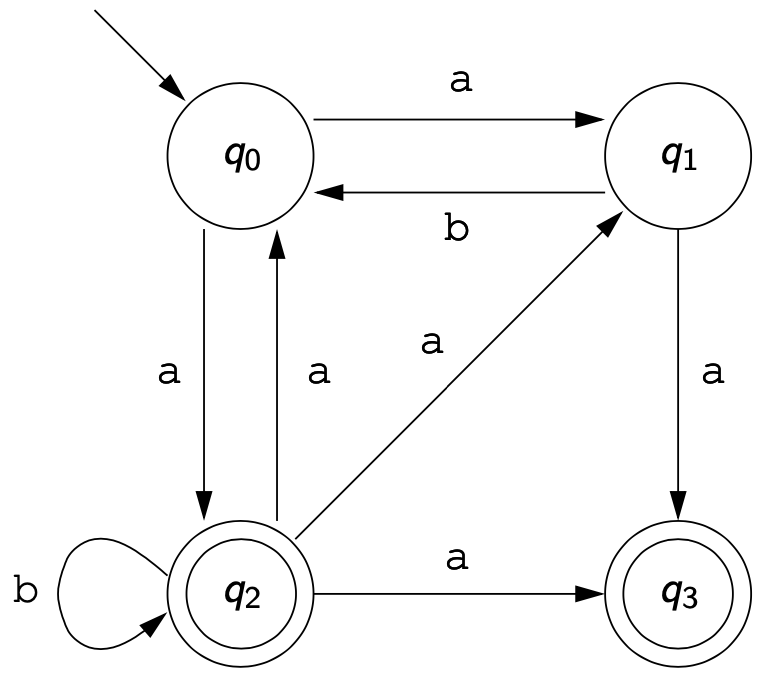
\includegraphics[width=\columnwidth]{reg-lang-7}
\end{figure}

\subsubsection{Equivalence of NFA and DFA}
We are going to prove shortly that for any NFA,
there exists a DFA which is equivalent, i.e. if
we consider the automata as black boxes,
we are not able to distinguish them
because they recognize the same language.
More formally, two finite state automata
$M_1$ and $M_2$ are equivalent if and only if they
recognize the same language, i.e. $L(M_1) = L(M_2)$.\\

The theorem states: \textit{For any nondeterministic finite state automaton NFA there exists a deterministic finite state automaton DFA, which is equivalent, and vice versa.}
From this theorem follows:
\begin{itemize}
  \item Non-determinism does not provide more expression power than determinism.
  \item NFA are generally more compact than equivalent DFA.
\end{itemize}
The first step of the proof is trivial, since any 
DFA is per definition a NFA (a deterministic FSA is a particular
case of a non-deterministic FSA).
The second step is not as easy as the first one.
In order to show that for any NFA there exists a 
DFA we are going to construct a DFA from the NFA and prove that both accept the same language.\\

Let $M = (Q, \Sigma, \delta, q_0, F)$ be a NFA. 
We construct a DFA $M' = (Q', \Sigma, \delta', q_0', F')$ as follows:
\begin{enumerate}
  \item $Q' = \mathcal{P}(Q)$. An element of $Q'$ will be denoted $[q_1,q_2,\dots,q_i]$
  where $q_1,\dots,q_i$ belong to $Q$. This element represents a single state of the deterministic automaton corresponding to a set of states of the NFA.
  \item $F'$ is the set of members of $Q'$ composed of at least one final state of $M$.
  \item $q_0' = [q_0]$
  \item $\delta'([q_1, \dots, q_i], s) = [p_1,\dots,p_j] \Longleftrightarrow \delta(\{q_1,\dots,q_i\}, s) = \{p_1,\dots,p_j\}$.
\end{enumerate}
Now we have to show that every word $w$ accepted by $M$ is also accepted by $M'$
and if $M$ does not accept the word $w$, then $M'$ rejects $w$.\\

We prove by induction on the length of $w$ that
\begin{align*}
  \delta^{\prime *}(q'_0, w) = [q_1,\dots,q_i] \\ \Longleftrightarrow \delta^{*}(\{q_0, w\}, s) = \{q_1,\dots,q_i\}
\end{align*}
\textit{Base case:} Trivial for $\lvert w \rvert = 0$ because
$q_0' = [q_0]$ and $w = \epsilon$.\\
\textit{Induction:} Let us assume that the above is true for some words of length $\leq m$.
Let $s \in \Sigma$ and $ws$ be a string of length $m+1$.
By definition of $\delta^{\prime *}$,
\begin{align*}
  \delta^{\prime *}(q_0', ws) = \delta'(\delta^{\prime *}(q_0', w), s).
\end{align*}
By induction hypothesis,
\begin{align*}
  \delta^{\prime *}(q'_0, w) = [p_1,\dots,p_j] \Longleftrightarrow \delta^{*}(q_0, w) = \{p_1,\dots,p_j\}.
\end{align*}
But by definition of $\delta'$,
\begin{align*}
  \delta'([p_1, \dots, p_j], s) = [r_1, \dots, r_k] \\ \Longleftrightarrow \delta (\{p_1, \dots, p_j\}, s) = \{r_1, \dots, r_k\}.
\end{align*}
Consequently, 
\begin{align*}
  \delta^{\prime *} (q_0', ws) = [r_1, \dots, r_k] \\ \Longleftrightarrow \delta^{*}(q_0, ws) = \{r_1, \dots, r_k\}.
\end{align*}
Finally, we only have to add the following $\delta^{\prime * }(q_0', w) \in F'$ only when
$\delta^{*}(q_0, w)$ contains a state of $Q$ that belongs to $F$. Thus,
$L(M) = L(M')$.\\

\textit{Example:} Here is a non-deterministic automaton. We eliminate the nondeterminism according to the method given in the proof of the theorem:
\begin{figure}[H]
  \centering
  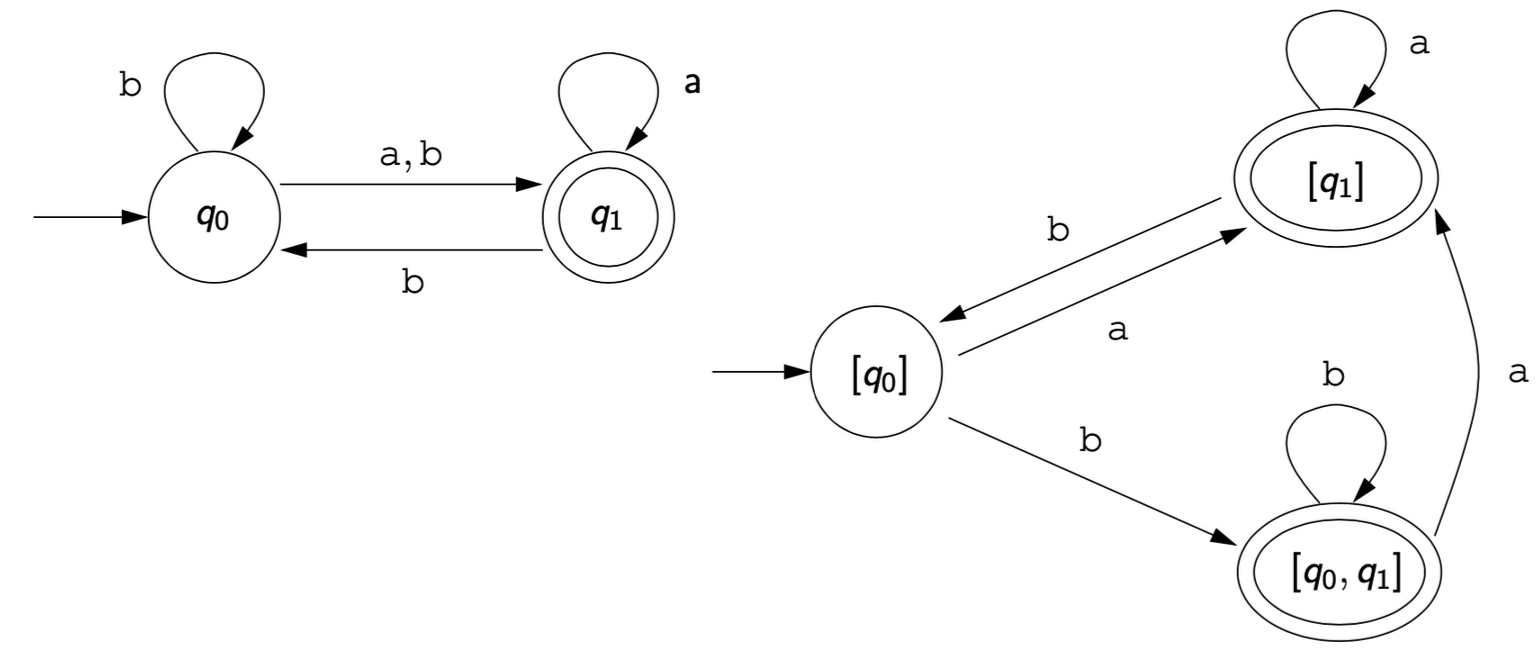
\includegraphics[width=\columnwidth]{reg-lang-8}
\end{figure}
\subsubsection{Automata with $\epsilon$-transitions}
Up to now, we have seen FSA where the label of the 
transition functions belong to the alphabet.
We can extend this so that we allow a transition to be caused 
by the empty string $\epsilon$.
Such transitions are called \textbf{$\epsilon$-transitions}, \textbf{empty transitions} or \textbf{spontaneous transitions}.
Empty transitions make the design and understanding of NFA easier.\\

A finite state automaton with $\epsilon$-transitions is defined 
in the same manner as a classic non-deterministic automata except that the
symbol $\epsilon$ is in the alphabet.\\

The concept of \textbf{$\epsilon$-closures} can be formally defined as follwing: For a state $q$ in $Q$ of an automaton $M$, the
$\epsilon$-closure($q$) is the set of all states of $M$
reachable from $q$ by a sequence of empty transitions:
\begin{align*}
  \epsilon\text{-closure}(q) & = \{p \in Q \vert (q,w) \vdash_m^{*}(p,w)\}\\
  \epsilon\text{-closure}(P) & = \bigcup_{p\in P} \epsilon\text{-closure}(q)
\end{align*}
where $P$ denotes a set of states.\\

For a given NFA with empty transitions,
we define a new transition function $\delta^{*}$
that uses the $\epsilon$-closure.
The new transition function is defined as follows:
\begin{enumerate}
  \item $\delta(q, \epsilon) = \epsilon\text{-closure}(q)$
  \item For every $w \in \Sigma^{*}$ and $s \in \Sigma$:
  \begin{align*}
    \delta^{*}(q, ws) = \epsilon\text{-closure}(P)
  \end{align*}
  where $P = \{p \vert p \in \delta{r, s}$ for an $r \in \delta^{*}(q,w)\}$
\end{enumerate}

We extend $\delta$ and $\delta^{*}$ for a set of states:
\begin{align*}
  \delta(R, s) & = \bigcup_{q \in R} \delta(q, s)\\
  \delta^{*}(R,w) & = \bigcup_{q \in R} \delta^{*}(q, w)
\end{align*}

The introduction of $\epsilon$-transitions
does not provide any extra expression power.
This means that for any NFA with $\epsilon$-transitions,
there exists a NFA without $\epsilon$-transitions.\\

The removal method of empty transitions of a non-deterministic
automaton consists of computing the $\epsilon$-closure for all states
of the automaton, which defines the transition function $\delta^{*}$.
Once the operation is performed, it is necessary to add the initial state
to the set of final states when the empty string is recognized
by the automaton with empty transitions.\\

\textit{Example:} Here is a non-deterministic automaton with 
some empty transitions:
\begin{figure}[H]
  \centering
  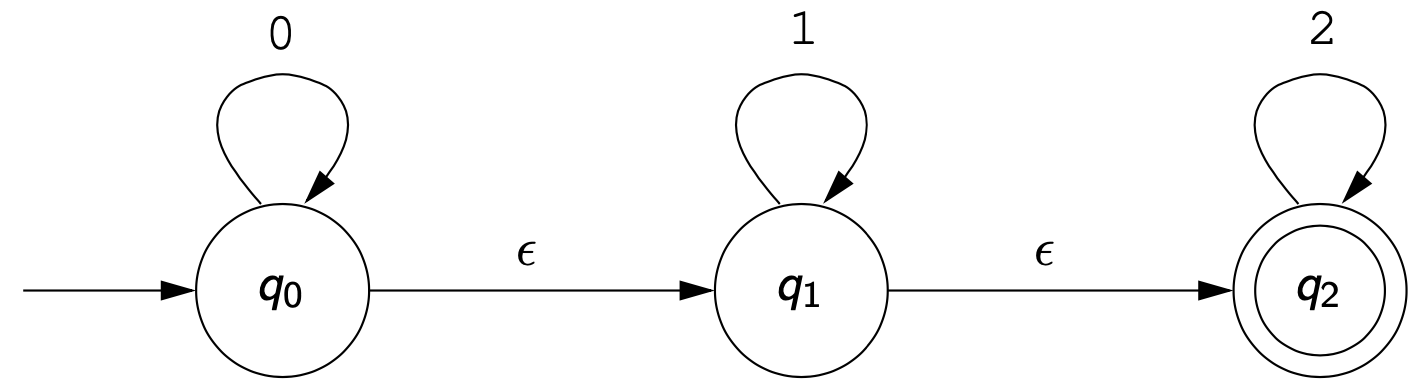
\includegraphics[width=\columnwidth]{reg-lang-9}
\end{figure}
The computation of the $\epsilon$-closure
provides the new transition function $\delta$:

\begin{table}[H]
  \centering
  \begin{tabular}{c | c | c | c} 
  $\delta$ & 0 & 1 & 2\\
  \hline
    $q_0$ & $\{q_0, q_1, q_2\}$ & $\{q_1, q_2\}$ & $\{q_2\}$\\
    $q_1$ & $\emptyset$ & $\{q_1, q_2\}$ & $\{q_2\}$\\
    $q_2$ & $\emptyset$ & $\emptyset$ & $\{q_2\}$
  \end{tabular}
\end{table}
All that remains now is to add $q_0$ to the 
set of final states since the empty string is
recognized by the above automaton:
\begin{figure}[H]
  \centering
  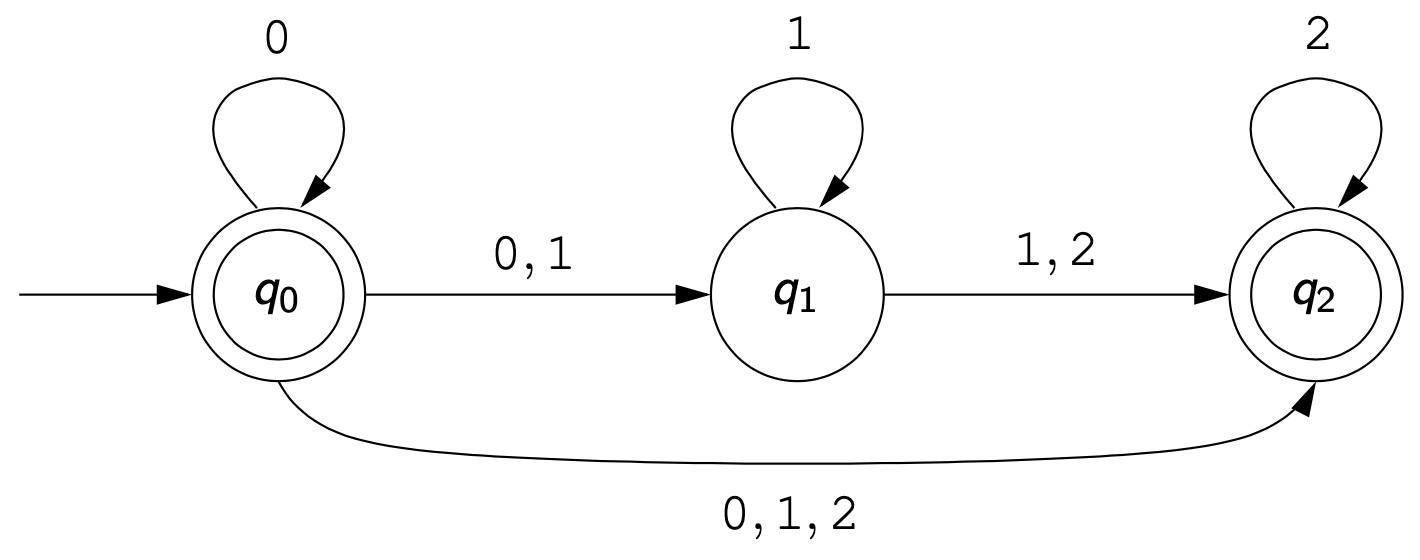
\includegraphics[width=\columnwidth]{reg-lang-10}
\end{figure}
Any language $L$ recognized by a NFA with $\epsilon$-tranistions
is also recognized by a NFA without $\epsilon$-transitions.

\subsubsection{Minimization of DFA}
% TODO: Self study.

\subsection{Properties of Regular Languages}
Regular languages have a few properties which are the following:
\begin{enumerate}
  \item The union $L_1 \cup L_2$ of two regular languages $L_1$ and $L_2$ is a regular language.
        Let $M_1$ and $M_2$ be two FSA such that $L(M_1) = L_1$ and $L(M_2) = L_2$.
        The union of both the languages recognized by the automata is a regular language.
        Indeed, we can construct an automaton that recognized $L_1$ and $L_2$ as follows:
        \begin{figure}[H]
          \centering
          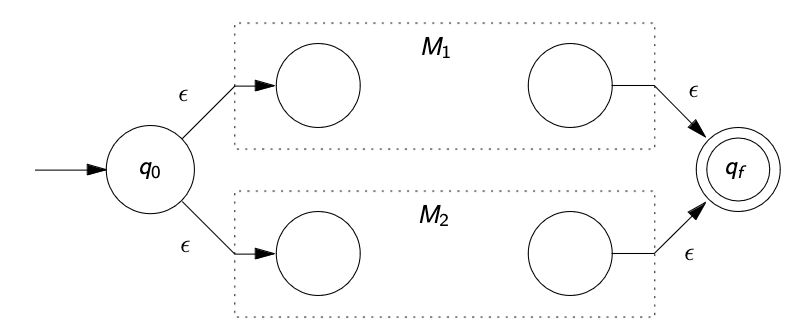
\includegraphics[width=\columnwidth]{reg-lang-11}
        \end{figure}
        If $w \in L_1$ (recognized by $M_1$) or $w \in L_2$ (recognized by $M_2$), then
        $w \in L_1 \cup L_2$ (recognized by the above FSA).
  \item The concatenation $L_1 \cdot L_2$ of two regular languages $L_1$ and $L_2$ is a regular language.
        \begin{figure}[H]
          \centering
          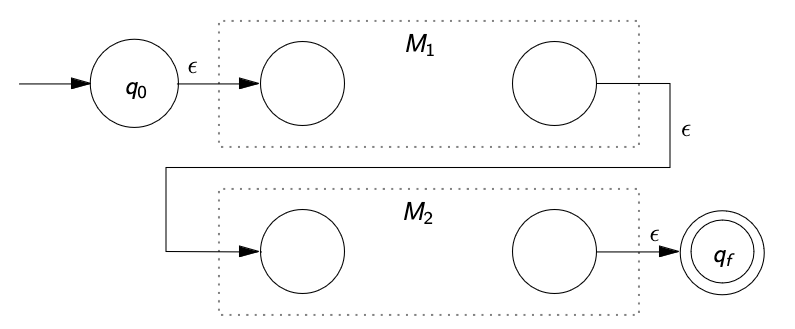
\includegraphics[width=\columnwidth]{reg-lang-12}
        \end{figure}
        If $w_1 \in L_1$ and $w_2 \in L_2$, then the concatenation $w_1 \cdot w_2 \in L_1 \cdot L_2$
        (recognized by the above FSA).
  \item The complementation $\overline{L} = \Sigma^{*} \backslash L$ of a regular language $L$ is a regular language as well.
        To construct an automaton accepting $\overline{L}$, it suffices to transform every final state into 
        a non-final state and every non-final state into a final state. The transition function must be total.
  \item The iterative closure $L^{*}$ of a language $L$ is a regular language.
        \begin{figure}[H]
          \centering
          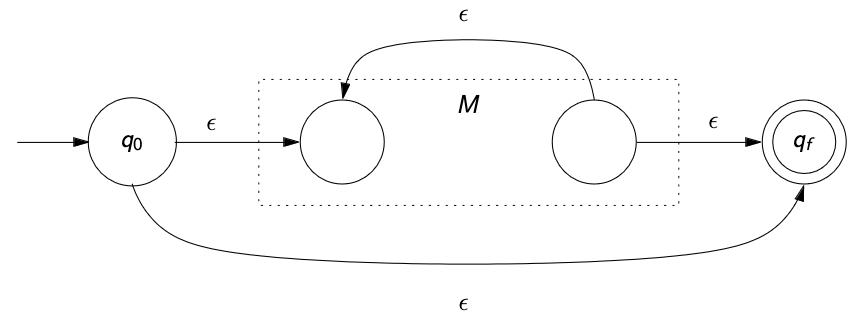
\includegraphics[width=\columnwidth]{reg-lang-13}
        \end{figure}
  \item The intersection $L_1 \cap L_2$ of two regular languages $L_1$ and $L_2$ is a regular language.
        Indeed, because
        \begin{align*}
          L_1 \cap L_2 = \overline{\overline{L_1} \cup \overline{L_2}}
        \end{align*}
        Previously, we saw that the complement of a regular language is regular (both $\overline{L_1}$ and $\overline{L_2}$ are regular)
        and the union of two regular languages is also regular as well as the last complementation. It follows that the intersection of two
        regular languages is regular.
\end{enumerate}
\subsection{Grammars}
\subsubsection{Introduction}
Just like the automata, a \textbf{grammar} is a formalism used for specifying languages.
Each grammar corresponds to a type of machine or automaton:
\begin{itemize}
  \item Regular grammars $\equiv$ finite state automata
  \item Context-free grammars $\equiv$ pushdown automata
  \item Grammars without restrictions $\equiv$ Turing machines
\end{itemize}
Intuitively, a grammar is a system of rules which allows to ``rewrite'' a term (or an expression)
into another term. Although the grammars and the FSA aare two similar formalisms,
there is a difference form an operational standpoint:
\begin{itemize}
  \item An automaton recognizes a language, i.e. consumes input symbols 
        and determines whether a word belongs to a language.
  \item A grammar on the other hand generates words.
\end{itemize}
Grammars are sometimes called rewriting systems and rules are called rewriting rules or productions.\\

A \textbf{rule} is composed of a \textbf{left-hand side} $\alpha$ and a \textbf{right-hand side} $\beta$ surrounding an arrow:
\begin{align*}
  \alpha \rightarrow \beta
\end{align*}
Both sides are composed of two types of symbols:
\begin{itemize}
  \item The \textbf{terminal} symbols that compose the words generated by the grammar.
  \item The \textbf{non-terminal} symbols that are mainly used in the rewriting process.
\end{itemize}
The rewriting of a term into another consists of applying a rule to the original term, i.e. to replace
the left-hand side which appears in the term with the right-hand side of the rule in order to obtain a new term.
Starting the rewriting process from a special rule called the \textbf{axiom} and applying repetitively the rules,
we obtain (not always) a term composed of a terminal symbol only (no more rules can be applied). Such a term 
is a word generated by the grammar.\\

The set of words generated by the rewriting process is called the language generated by the grammar.
The rewriting process can be endless and corresponds to a computer program which does not terminate.
Since any rules can be selected during the rewriting process, the rewriting process is potentially 
non-deterministic.\\

The formal definition of a grammar is as follows: A grammar is a 4-tuple $G = (V_T, V_N, P, S)$, where 
\begin{itemize}
  \item $V_T$ is a set of terminal symbols
  \item $V_N$ is a set of non terminal symbols such that $V_T \cap V_N = \emptyset$
  \item $P$ is a set of rules $\alpha \rightarrow \beta$, where $\alpha$ and $\beta$ are sequences
        of terminals or non-terminals, but $\alpha$ must contain at least non-terminal
  \item $S \in V_N$ is the axiom or the initial symbol
\end{itemize}
Let $G = G = (V_T, V_N, P, S)$ be a grammar and $A \rightarrow B$
a production of $P$. The sequence of terminals and non-terminals $\alpha A\beta \in (V_T \cup V_N)^{*}$
can be derived into a sequence $\alpha B\beta$ by applying the production $A \rightarrow B$,
i.e. by substituting $A$ for $B$. We call the move from a sequence $\alpha$ to another sequence $\beta$
by applying one production of the grammar a \textbf{one-step-derivation}.
We denote this derivation $\alpha \Rightarrow_G \beta$. We call a \textbf{derivation} a sequence of one-step
derivations and denote such a derivation $\alpha \Rightarrow_G^{*}\beta$.\\

The formal definition of a language generated by a grammar is as follows:
The language $L(G)$ generated by a grammar $G = (V_T, V_N, P, S)$ is the set
of all words which can be optained or derived by rewriting from the axiom $S$ 
and do not contain any terminals:
\begin{align*}
  L(G) = \{w \mid S \Rightarrow_G^{*} w, w \in V_T^{*}\}
\end{align*}
\textit{Examples:}
\begin{enumerate}
  \item The grammar
        \begin{align*}
          G = (\{a,b\}, \{S,A\}, P, S)
        \end{align*}
        in which
        \begin{align*}
          P = \{S \rightarrow bbA, A \rightarrow aaA, A \rightarrow aa\}
        \end{align*}
        generates the language
        \begin{align*}
          L(G) = \{bb\} \cdot \{aa\}^{n} \text{ where $n \geq 1$.}
        \end{align*}
  \item The (regular) grammar
        \begin{align*}
          G = (\{0,1\}, \{S\}, P, S)
        \end{align*}
        where
        \begin{align*}
          P = \{S \rightarrow 1S, S \rightarrow 0S, S \rightarrow 1\}
        \end{align*}
        generates
        \begin{align*}
          L(G) = \{0,1\}^{*} \cdot \{1\}.
        \end{align*}
  \item The (context-free) grammar
        \begin{align*}
          G = (\{a,b\}, \{S\}, P, S)
        \end{align*}
        where
        \begin{align*}
          P = \{S \rightarrow aSb, S \rightarrow \epsilon\}
        \end{align*}
        generates
        \begin{align*}
          L(G) = \{a^nb^n \mid n \geq 0\}.
        \end{align*}
        The empty string $\epsilon$ means that a term can be replaced by a string of length zero.
  \item The language $L = \{a^nb^nc^n \mid n \geq 1\}$ is generated by the grammar
        \begin{align*}
          G = (\{a,b,c\}, \{S,A,B,C,D\}, P, S)
        \end{align*}
        where
        %\begin{align*}
          $P = \{S \rightarrow aACD, A \rightarrow aAC, A \rightarrow \epsilon, B \rightarrow b,
          CD \rightarrow BDc, CB \rightarrow BC, D \rightarrow \epsilon
          \}.$
        %\end{align*}
        This grammar is neither regular nor context-free.
\end{enumerate}
\subsubsection{Regular Grammar}
We formally define \textbf{regular grammars} as follows:
A grammar is \textbf{right-regular} if all rewriting rules have the form
$\alpha \rightarrow \beta$ with the following restrictions:
\begin{enumerate}
  \item $\lvert \alpha \rvert = 1, \alpha \in V_N$
  \item $\beta = aB, \beta = a, \text{ or } \beta = \epsilon \text{ with } B \in V_N \text{ and } a \in V_T$
\end{enumerate}
A grammar is \textbf{left-regular} if all productions have the form:
\begin{enumerate}
  \item $\lvert \alpha \rvert = 1, \alpha \in V_N$
  \item $\beta = Ba, \beta = a, \text{ or } \beta = \epsilon \text{ with } B \in V_N \text{ and } a \in V_T$
\end{enumerate}
Any right or left-regular grammar us simply called a regular grammar.\\

It is important to note that a regular grammar is either left regular or right regular, but not both (except for the trivial cases).
If the rules of right and left-regular grammars are mixed, then the language generated by the grammar can be non-regular.
Non-regular grammars generate more complex languages than regular ones.\\

FSA and regular grammars are equivalent: A language $L$ is recognized by a FSA iff $L$ is generated by a regular grammar.
% TODO: Proof?

\subsubsection{Regular Expressions}
\textbf{Regular expressions} are the third formalism after FSA and regular grammars that can be used 
to specify regular languages. We say that a regular expression \textbf{denotes} a regular language
(automata recognized and grammars generate). Regular expressions are easy to integrate into
software systems and are widely used for searching sub-strings in text, 
for instance in editors or web search engines.
Regular expressions are also intensively used for syntax analysis and consequently for compiler design.\\

The formal definition of a regular expression is as follows: Let $\Sigma$ be an alphabet.
A regular expression defined over $\Sigma$ is recursively defined as follows:
\begin{enumerate}
  \item $\emptyset$ us a regular expression that denotes the empty set
  \item $\epsilon$ is a regular expression that denotes the set $\{\epsilon\}$
  \item For any $a \in \Sigma$, $a$ is a regular expression that denotes the set $\{a\}$
  \item If $r$ and $s$ are two regular expressions which denote the sets $R$ and $S$ respectively
        then $(r + s)$, $(rs)$ and $(r^{*})$ are regular expressions that denote the sets
        $R \cup S$, $R \cdot S$ and $R^{*}$.
  \item Nothing else is considered a regular expression
\end{enumerate}
The language denoted by a regular expression $r$ is written $L(r)$.\\

\textit{Examples:}
\begin{enumerate}
  \item Let $\Sigma = \{a,b\}$ and the regular expression
        \begin{align*}
          r = (a ( a + b)^{*})
        \end{align*}
        then
        \begin{align*}
          L(r) = \{a\} \cdot \{a,b\}^{*}.
        \end{align*}
  \item The regular expression
        \begin{align*}
          r = (0^{*}1)^{*} + 0
        \end{align*}
        denotes the set
        \begin{align*}
          L(r) = ({0}^{*} \cdot \{1\})^{*} \cup \{0\}
        \end{align*}
        or
        \begin{align*}
          & L(r) = \{x \mid x \in \{0,1\}^{*} \text{,}\\
          & \text{$x$ represents an} \\
          & \text{ odd binary number }\}\\
          & \cup \{\epsilon\}.
        \end{align*}
    \item The regular expression
          \begin{align*}
            r = (a(ab)* (a+ \epsilon))^{*}
          \end{align*}
          corresponds to the automaton $M$:
          \begin{figure}[H]
            \centering
            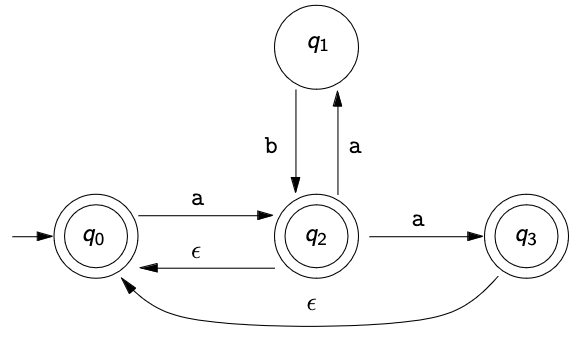
\includegraphics[width=\columnwidth]{reg-lang-14}
          \end{figure}
\end{enumerate}
The following equalities hold for regular expressions:
\begin{itemize}
  \item $r + s = s + r$
  \item (r + s) + t = r + (s + t)
  \item $(rs)t = r(st)$
  \item $r(s + t) = rs + rt$
  \item $(r + s)t = rt + st$
  \item $\emptyset^{*} = \epsilon$
  \item $(r^{*})^{*} = r^{*}$
  \item $(\epsilon + r)^{*} = r^{*}$
  \item $(r^{*} s^{*})^{*} = (r+s)^{*}$
\end{itemize}
Regular expressions are equivalent to FSA: 
\begin{itemize}
  \item Regular expressions to FSA: From any regular expression $r$, there exists a NFA
  with $\epsilon$-transitions which recognizes $L(r)$. 
  \item DFA to regular expressions: If a language $L$ is recognized by a DFA, then there exists a regular
        expression $r$ that denotes $L$.
\end{itemize}
